\chapter{Introduzione alla Modellizzazione}

\begin{wrapfigure}{r}{0.5\textwidth}
  \begin{center}
    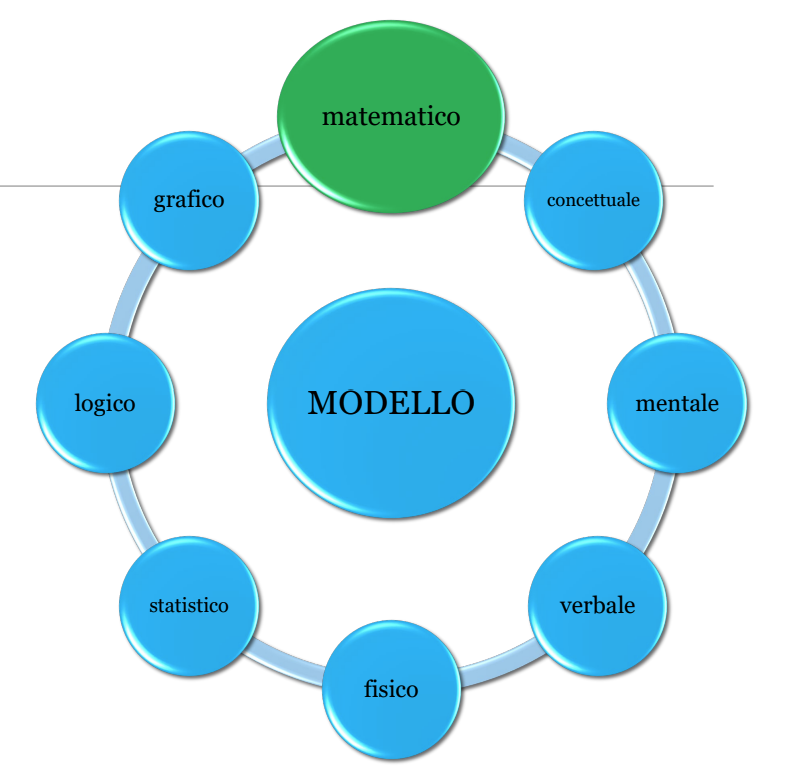
\includegraphics[width=0.5\textwidth]{immagini/tipidimodelli.png}
  \end{center}
\end{wrapfigure}
In ambito biologico e bioingegneristico, un \textbf{modello} può essere definito come una rappresentazione della realtà caratterizzata da un preciso livello di approssimazione. A seconda delle necessità e degli strumenti utilizzati, un modello può assumere diverse forme: può essere concettuale, mentale, verbale, fisico, statistico, logico, grafico o matematico. 

Per comprendere la differenza tra queste tipologie, si consideri l'esempio dell'assorbimento di un farmaco nel sangue. 
\begin{itemize}
    \item \textbf{Modello grafico} rappresenterà visivamente la concentrazione plasmatica del farmaco nel tempo (ad esempio, evidenziando una curva di decadimento esponenziale che descrive un'eliminazione di primo ordine in scala lineare).
    \item \textbf{Modello matematico}, invece, formalizzerà il medesimo processo attraverso un'equazione differenziale, come ad esempio:
\end{itemize}

\medskip
\begin{equation}
\frac{dC}{dt} = -kC
\end{equation}
dove $C$ rappresenta la concentrazione e $k$ la costante di eliminazione.

Il livello di dettaglio di un modello è fondamentale e deve essere sempre bilanciato. Un modello realistico del sistema circolatorio umano, ad esempio, dovrebbe teoricamente descrivere matematicamente il comportamento di ogni singola cellula cardiaca. Tuttavia, un simile livello di dettaglio porterebbe a un sistema di equazioni di dimensioni intrattabili e, di fatto, irrisolvibile. La soluzione risiede nella \textbf{semplificazione}: è possibile scrivere un'equazione per ogni camera cardiaca. Questo introduce un'approssimazione della realtà, ma il livello di dettaglio rimane sufficiente per descrivere correttamente e utilmente il fenomeno macroscopico del pompaggio del sangue.

\section{Obiettivo e Categorie dei Modelli Matematici}

Il modo in cui un modello viene formulato e il livello di dettaglio adottato dipendono principalmente dall'\textbf{obiettivo} del modello stesso. L'obiettivo guida la transizione dal sistema reale alla scelta della metodologia di modellizzazione, fino alla realizzazione del modello finale.
\begin{figure}[h]
    \centering
    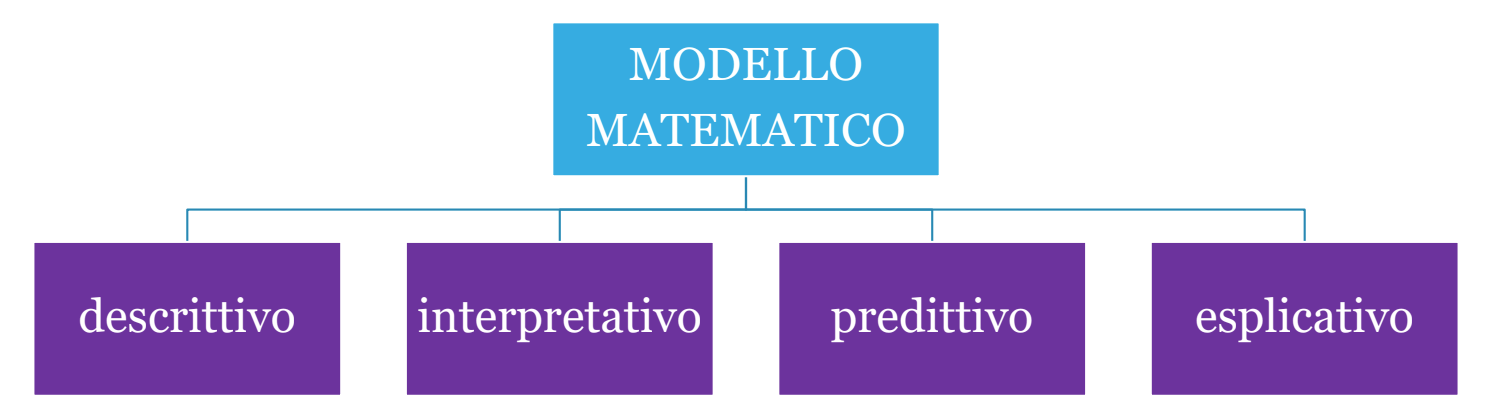
\includegraphics[width=1\linewidth]{immagini/itipidimodello.png}
\end{figure}

\noindent I modelli matematici possono essere suddivisi in quattro categorie principali in base al loro scopo:

\begin{itemize}
    \item \textbf{Descrittivi:} Sono utilizzati per esprimere relazioni quantitative in modo conciso attraverso le equazioni. Questo facilita notevolmente l'analisi e il trattamento dei dati. Ad esempio, se due variabili di un sistema sono direttamente proporzionali, è molto più semplice ed elegante esprimerle tramite un'equazione lineare piuttosto che ricorrere a descrizioni verbali o grafiche.
    \item \textbf{Interpretativi:} Servono a interpretare i dati raccolti o i risultati sperimentali. Riprendendo l'esempio dell'assorbimento di un farmaco nel flusso sanguigno, una curva di decadimento esponenziale rappresenta in modo compatto dei dati che approssimano un processo di primo ordine, permettendo di estrarre parametri utili come la velocità di comparsa (rate of appearance) dall'argomento dell'esponenziale. Permette di spiegare meglio il fenomeno.
    \item \textbf{Predittivi:} Sono impiegati per prevedere come il sistema risponderà a uno stimolo o a un cambiamento interno. Sono lo strumento principe per le \textit{simulazioni}. Ad esempio, conoscendo il modello di un organismo, è possibile simulare l'infusione di un farmaco e valutarne a priori l'effetto terapeutico.
    \item \textbf{Esplicativi:} Hanno l'obiettivo di far comprendere i meccanismi intimi di un fenomeno. In questi modelli, i parametri matematici corrispondono a specifici processi fisiologici; variando tali parametri, è possibile osservare come muta il comportamento globale del sistema, permettendo, ad esempio, la simulazione di comportamenti patologici (come l'attività di neuroni epilettici).
\end{itemize}
Oltre a questi scopi primari, i modelli trovano impiego nella valutazione di ipotesi alternative (confrontando l'accuratezza di vari modelli rispetto a dati reali), nell'inferenza di misure che non possono essere prelevate in vivo, nell'assistenza ai processi educativi (tramite simulatori) e nell'aiuto alla pianificazione sperimentale (ad esempio, definendo gli istanti ottimali per i prelievi di sangue in uno studio di farmacocinetica).
\newpage
\section{Approcci alla Modellizzazione}

Esistono due macro-approcci per modellare un sistema biologico: i modelli basati sui dati e i modelli basati sul sistema fisiologico.

\subsection{Modello dei dati (Data-driven o Black-box)}
Questi modelli forniscono una descrizione quantitativa ricavata puramente dall'analisi dei dati sperimentali di ingresso e uscita (input/output) prelevati dal sistema, senza indagare i meccanismi interni (approccio \textit{black-box}). Esempi tipici sono i sistemi lineari tempo-invarianti (LTI) o le reti neurali artificiali. 
Il modello dei dati dal punto di vista delle procedure di modellizzazione è piu semplice. Il processo di modellizzazione prevede \textbf{due step}: 
\begin{itemize}
    \item Definizione di una rappresentazione input/output del modello: dobbiamo definire le equazioni matematiche (struttura del modello) con cui vogliamo fittare i dati e il grado di complessità del formalismo matematico alla base del modello.
    \item Stima dei parametri: misura dei dati dal sistema sottoponendolo a degli ingressi. Si fa quello che viene chiamato “processo di identificazione” o “stima dei parametri”, sostanzialmente si usano i dati raccolti dal sistema per dare dei valori ai parametri incogniti.
\end{itemize}
Ad esempio possiamo dire che $y=f(u,p)$ dove $y$ è l'uscita, $u$ l'ingresso e $f$ il parametro incognito. Il modello descrittivo, interpretativo e predittivo ricadono all'interno della definizione di modello di dati.
\begin{figure}[h]
    \centering
    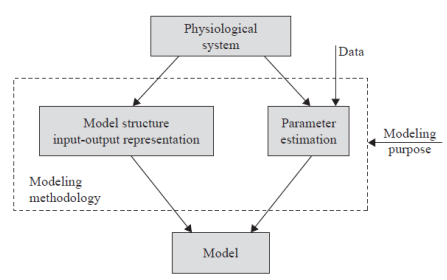
\includegraphics[width=0.5\linewidth]{immagini/modellodatidiagramma.png}
\end{figure}

\subsection{Modello del sistema}
Questo approccio tenta di rappresentare esplicitamente la fisiologia alla base del sistema (ad esempio tramite modelli a compartimenti o circuiti equivalenti). Pur costituendo sempre un'approssimazione della realtà, offre il grande vantaggio di utilizzare variabili e parametri che sono direttamente correlati alle dinamiche e alle proprietà fisiche o biologiche del sistema stesso.
Il processo di formulazione in questo caso è più articolato:
\begin{enumerate}
    \item Formulazione del modello concettuale.
    \item Realizzazione matematica (traduzione in equazioni).
    \item Identificazione a priori dei parametri basata sulle conoscenze fisiche del fenomeno.
    \item Stima o raffinamento dei parametri tramite i dati del sistema.
    \item Soluzione del modello e implementazione computazionale per legare le variabili di interesse.
\end{enumerate}
Il modello esplicativo ricade sicuramente nel modello del sistema; tuttavia, possiamo considerare anche il modello predittivo come modello di sistema (se correlato alle dinamiche fisiche/ biologiche del sistema).
\begin{figure}[h]
    \centering
    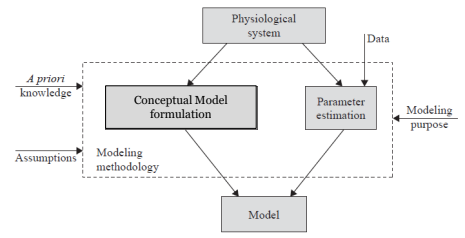
\includegraphics[width=0.55\linewidth]{immagini/modellodelsistema.png}
\end{figure}
\section{L'Approssimazione della Realtà}
Poiché nessun modello può replicare la realtà nella sua interezza, è necessario ricorrere a specifiche tecniche di approssimazione:
\begin{itemize}
    \item \textbf{Aggregazione:} Consiste nell'accorpare parti del sistema reale in macro-elementi. Un esempio classico è la modellizzazione dello spazio extravascolare come un unico grande compartimento, oppure la rappresentazione del rene come singolo blocco anziché modellarne i singoli nefroni.
    \item \textbf{Astrazione:} Prevede di includere nel modello soltanto gli aspetti del sistema che sono pertinenti allo studio. In un modello sulla regolazione del glucosio, ad esempio, si assume che nel circolo sanguigno vi siano solo il glucosio e gli ormoni strettamente correlati ad esso (come l'insulina), ignorando il resto degli elementi ematici.
    \item \textbf{Idealizzazione:} Strutture o comportamenti complessi e difficili da tradurre in formule vengono idealizzati. Ad esempio, si può ipotizzare che un farmaco iniettato si distribuisca istantaneamente e uniformemente in tutto l'organismo, trascurando il transitorio di diffusione.
\end{itemize}
\newpage
\section{Identificazione e Validazione del Modello}
\subsection{Identificazione del modello}

\begin{wrapfigure}{r}{0.5\textwidth}
  \begin{center}
    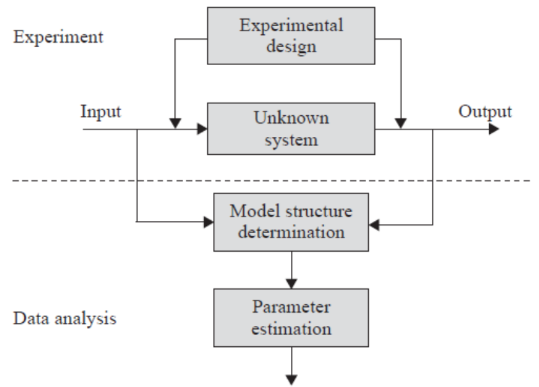
\includegraphics[width=0.5\textwidth]{immagini/indentificazionedelmodello.png}
  \end{center}
\end{wrapfigure}
La transizione dal sistema reale al modello matematico richiede l'esatta definizione della struttura e la determinazione numerica di tutti i suoi parametri. Questo processo, chiamato \textbf{identificazione}, si nutre di dati empirici: confrontando l'uscita misurata con l'uscita del modello si aggiustano i parametri fino a che l'uscita del modello
diviene il più possibile vicina alla misura fatta. I dati possono essere intrinseci al sistema (es. segnali neurali o cardiaci) oppure derivare da esperimenti ad-hoc in cui si applicano stimoli noti (somministrazione di traccianti, variazioni dei gas inspirati) e si misurano le risposte.

\medskip 
\noindent Sorge in questa fase il \textbf{problema dell'identificabilità a priori}: i dati a disposizione sono sufficienti a stimare in modo univoco i parametri del modello? Spesso si assiste a un mismatch tra la complessità del modello scelto e la reale disponibilità di dati. Se il modello possiede troppi parametri rispetto ai dati, occorre semplificarne la struttura (riduzione dell'ordine) oppure arricchire il design sperimentale (acquisendo più campioni o stimolando il sistema in modo diverso). Se invece il modello risulta univocamente identificabile, si procede alla stima formale, tipicamente tramite l'approccio dei minimi quadrati (lineari o non lineari).

\subsection{Validazione}
La validazione ha lo scopo di misurare la bontà del modello rispetto agli obiettivi prefissati e di selezionare il migliore tra modelli alternativi. Si tratta di un processo iterativo: se il modello fallisce i test di validazione, è necessario tornare indietro, modificarne la struttura o le assunzioni, e ripetere l'identificazione.

\noindent I criteri di validazione differiscono dai metodi di stima e includono:
\begin{itemize}
    \item \textbf{Analisi dei residui:} Valutazione quantitativa dell'errore (mismatch) tra l'uscita prodotta dal modello e i dati empirici.
    \item \textbf{Plausibilità fisiologica:} Verifica che i parametri stimati (se il modello è di tipo esplicativo/fisiologico) ricadano in range biologicamente o fisicamente sensati.
    \item \textbf{Parsimonia:} A parità di accuratezza predittiva, va sempre scelto il modello con il minor numero di parametri.
\end{itemize}
\begin{figure}[h]
    \centering
    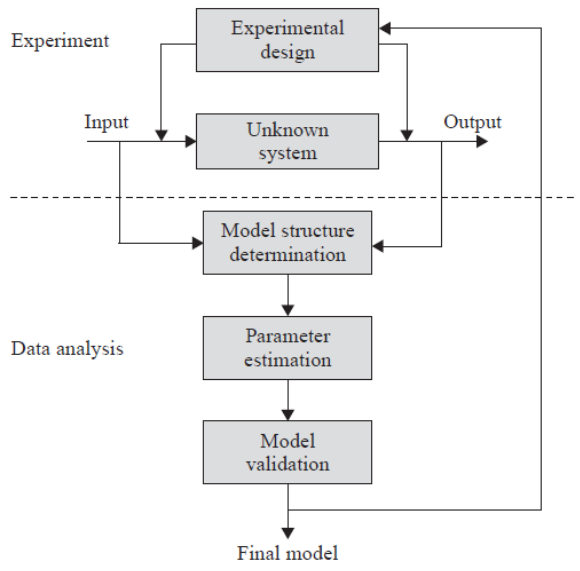
\includegraphics[width=0.5\linewidth]{immagini/validazionedelmodello.png}
\end{figure}

\newpage
\section{Soluzione e Simulazione}

L'ultimo passo della modellizzazione prevede la \textbf{soluzione} delle equazioni. Quando possibile, si ricercano soluzioni analitiche in forma chiusa, ma più frequentemente — a causa delle non-linearità e dell'elevato numero di variabili — è necessario ricorrere a metodi di ottimizzazione e integrazione numerica tramite computer.

Una volta risolto e validato, il modello diviene un simulatore a tutti gli effetti. La \textbf{simulazione} fornisce informazioni preziose, permette di prevedere comportamenti inesplorati e può portare a nuove scoperte. Soprattutto, la simulazione al calcolatore costituisce un'alternativa irrinunciabile all'esperimento sul sistema reale ogniqualvolta quest'ultimo risulti inaccessibile, pericoloso per il paziente, eticamente scorretto, eccessivamente costoso o temporalmente impraticabile.